\documentclass{article}

\usepackage{lipsum}
\usepackage[margin=1in,includefoot]{geometry}
\usepackage{graphicx}
\usepackage{float}
\usepackage[hidelinks]{hyperref}
\usepackage{amsmath}
\usepackage{amssymb}
\usepackage{color}

\usepackage[usenames,dvipsnames]{xcolor}
\usepackage{listings}
\lstset {language=C++}

% Header and Footer Stuff
\usepackage{fancyhdr}
\pagestyle{fancy}
\fancyhead{}
\fancyfoot{}
\fancyfoot[R]{\thepage}
\renewcommand{\headrulewidth}{0pt}
\renewcommand{\footrulewidth}{0pt}

\definecolor{dkgreen}{rgb}{0,0.6,0}
\definecolor{gray}{rgb}{0.5,0.5,0.5}
\definecolor{mauve}{rgb}{0.58,0,0.82}

\lstset{
  language=C++,
  aboveskip=3mm,
  belowskip=3mm,
  showstringspaces=false,
  columns=flexible,
  basicstyle={\small\ttfamily},
  numbers=none,
  numberstyle=\tiny\color{gray},
  keywordstyle=\color{blue},
  commentstyle=\color{dkgreen},
  stringstyle=\color{mauve},
  breaklines=true,
  breakatwhitespace=true,
  tabsize=3
}


\begin{document}

\begin{titlepage}
	\begin{center}
	\begin{align*}
	
\includegraphics[height=1.75in]{logo.png}
	\end{align*}


	
	\line(1,0){300}\\
	[0.25in]
	\huge{\bfseries Tutorial 4 }\\
	[2mm]
	\line(1,0){200}\\
	[1.5cm]
	\textsc{\LARGE Hierarchy}\\
	[0.75cm]
	\textsc{\Large CS4052 Computer Graphics}\\
	[7cm]	
	\end{center}
	
	\begin{flushright}
	\textsc{\large Alexandru Sulea\\
	D Stream\\
	\#12315152\\
	29 October 2016\\}
	\end{flushright}
	
\end{titlepage}
%Table of Contents Stuff%
%\tableofcontents
%\listoffigures
%\addcontentsline{toc}{section}{List of Figures}
%\listoftables
%\addcontentsline{toc}{section}{List of Tables}


\thispagestyle{empty}
\cleardoublepage
\pagenumbering{arabic}
\setcounter{page}{1}

\pagebreak
\section{Overview}
For this project I primarily used the code that was provided for the tutorial and followed the instructions set out in the handout sheet. The only bit of code that is repetitive is the translation commands with color change which I took from the second tutorial. I chose to reuse this methadology because it helps show you if there is a problem with the keyboard command or the translation command.

\section{Five Teapots}
For this tutorial, I chose to use 8 teapots, keeping the two teapots provided by the tutorial and adding 6 more to the scene.\\
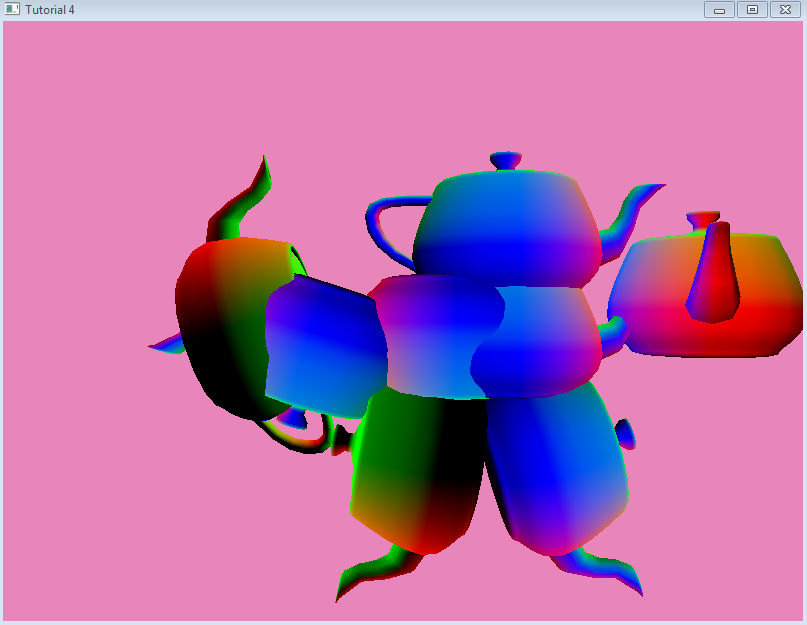
\includegraphics[height=2in,width=5in]{tut41.PNG}



\section{One-to-One Relationship}
For one to one relationship I chose the left arm to the left hand. The left hand can be rotated with respect to the left arm.
\begin{lstlisting}
	/*7 -  left arm*/
	mat4 local7 = identity_mat4();
	local7 = rotate_y_deg(local7, 0);
	local7 = rotate_x_deg(local7, 0);
	local7 = rotate_z_deg(local7, rotate7z);
	local7 = translate(local7, vec3(-14.0, -3.0, translate7z));
	mat4 global7 = global1*local7*local4;
	// update uniform & draw
	glUniformMatrix4fv(matrix_location, 1, GL_FALSE, global7.m);
	glDrawArrays(GL_TRIANGLES, 0, teapot_vertex_count);

	/*8 -  left hand*/
	mat4 local8 = identity_mat4();
	local8 = rotate_y_deg(local8, 180);
	local8 = rotate_x_deg(local8, 0);
	local8 = rotate_z_deg(local8, rotate8z);
	local8 = translate(local8, vec3(5, -3.0, translate8z));
	mat4 global8 = global7*local8;
	// update uniform & draw
	glUniformMatrix4fv(matrix_location, 1, GL_FALSE, global8.m);
	glDrawArrays(GL_TRIANGLES, 0, teapot_vertex_count);

	/*END*/
	glutSwapBuffers();
}
\end{lstlisting}

\section{One-to-Many Relationship}
The one to many relationship si between the right arm teapot and the rest of the teapots. The right arm teapot acts as the body of the manechin and thus all other manechins rotate and translate with respect to it.

\begin{lstlisting}
mat4 global3 = global1*local3;
mat4 global4 = global1*local4;
mat4 global5 = global1*local5;
mat4 global6 = global1*local6;
\end{lstlisting}


\section{Keyboard Control}
For keyboard control I used the wasd system for translations and a few other for moving the head of the manechin left and right.
\begin{lstlisting}
	float color()
	{
		float r = ((double)rand() / (RAND_MAX));
		float g = ((double)rand() / (RAND_MAX));
		float b = ((double)rand() / (RAND_MAX));
		return red = r, green = g, blue = b;
	}
	local1 = translate(local1, vec3(8.0+translate1x, translate1y, -60.0f+translate1z));
	mat4 global1 = local1;
	if (key == 'd') {
		color();
		translate1x = translate1x + temp;
		printf("%f", translate1x);
	}
\end{lstlisting}



\section{Unusual Structure}
For my structure I chose to have a manechin made of 8 teapots, i chose this model because I believe it will greatly aid me in the next tutorial.
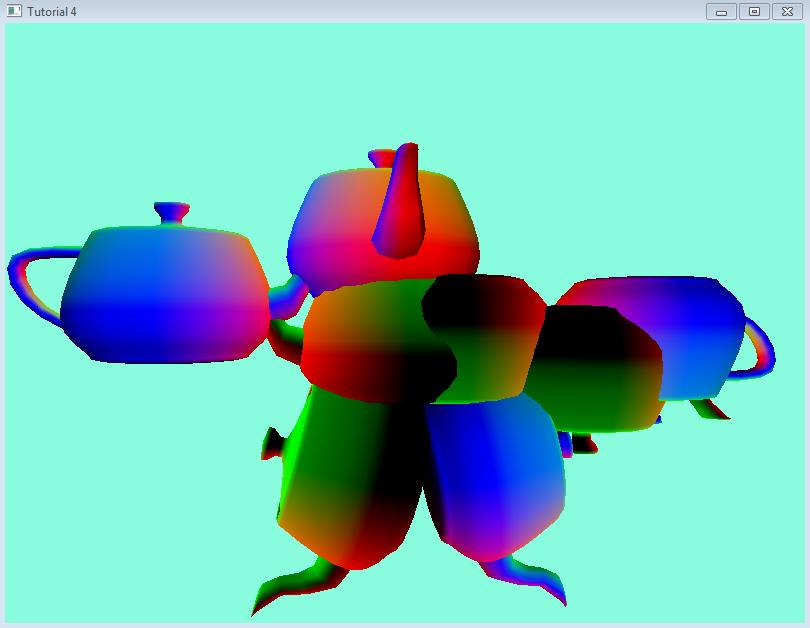
\includegraphics[height=2in,width=5in]{42.PNG}
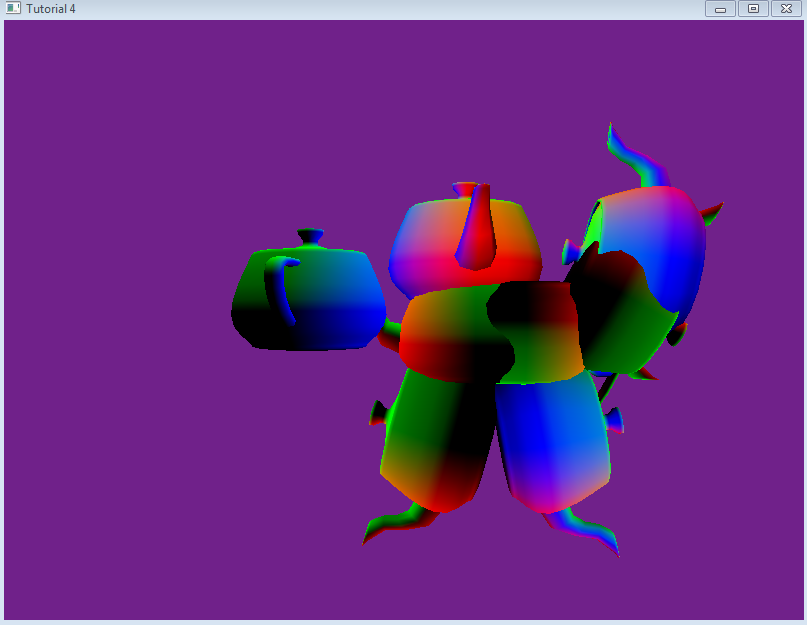
\includegraphics[height=2in,width=5in]{43.PNG}





	
\end{document}